\documentclass{article}
\pagestyle{plain}
\usepackage[a4paper, margin=.8in]{geometry}

\usepackage{amssymb}
\usepackage{varwidth}
\usepackage{siunitx}
\usepackage{amsmath}
\usepackage{multicol}
\usepackage{bm}
\usepackage{pdfpages}

\usepackage[utf8]{inputenc}
\usepackage{t1enc}
\def\magyarOptions{defaults=hu-min}
\usepackage[magyar]{babel}

\usepackage{graphicx}
\graphicspath{ {./} }

\usepackage{pgf}
\usepackage{tikz}
\usepackage{pgfplots}
\pgfplotsset{compat=1.18}
\usetikzlibrary {arrows.meta, decorations.markings, calc, patterns, pgfplots.fillbetween}

\usepackage{fancyhdr}
\fancypagestyle{plain}{%
	\fancyhf{}%

	\fancyhead{}
	\fancyhead[L]{Vári Gergő}
	\fancyhead[C]{MQHJ0H}
	\fancyhead[R]{\includegraphics[scale=.25]{signature}}
	\setlength{\headheight}{16.5pt}

	\fancyfoot{}
	\fancyfoot[C]{\thepage}
}

\title{Statika 4. HF}
\author{Vári Gergő}
\date{
	\parbox{\linewidth}{
		\centering
		\today\endgraf\bigskip
		\includegraphics[scale=.4]{shear}
	}
}

\pgfmathsetmacro{\a}{0.6}
\pgfmathsetmacro{\b}{0.6}
\pgfmathsetmacro{\c}{0.5}
\pgfmathsetmacro{\k}{0.1}
\pgfmathsetmacro{\p}{5}
\pgfmathsetmacro{\Fp}{\p * (\b+\c)}
\pgfmathsetmacro{\F}{4}

\pgfmathsetmacro{\Ay}{\Fp - \F}
\pgfmathsetmacro{\Cy}{-\Ay}
\pgfmathsetmacro{\Ma}{\Ay * \a}
\pgfmathsetmacro{\Bx}{(\F * \b - \p * ((\b+\c)/2))/\k}
\pgfmathsetmacro{\Cx}{\Bx}
\pgfmathsetmacro{\Ax}{-\Cx}

\newcommand{\pnum}[1]{%
	\pgfmathprintnumber[fixed]{#1}
}

\begin{document}


\pgfmathsetmacro{\unitm}{8}
\pgfmathsetmacro{\shownm}{1/8}
\pgfmathsetmacro{\unitkn}{1/3}
\pgfmathsetmacro{\shownkn}{3}

\pgfmathsetmacro{\a}{0.6}
\pgfmathsetmacro{\b}{0.6}
\pgfmathsetmacro{\c}{0.5}
\pgfmathsetmacro{\k}{0.1}
\pgfmathsetmacro{\p}{5}
\pgfmathsetmacro{\F}{4}

\pgfmathsetmacro{\as}{\a * \unitm}
\pgfmathsetmacro{\bs}{\b * \unitm}
\pgfmathsetmacro{\cs}{\c * \unitm}
\pgfmathsetmacro{\ks}{\k * \unitm}

\pgfmathsetmacro{\ps}{\p * \unitkn}
\pgfmathsetmacro{\Fs}{\F * \unitkn}

\newcommand{\struccoordsys}{%
	\draw[thick,->] (0,0) -- ++(1,0) node[anchor=north west] {x};
	\draw[thick,->] (0,0) -- ++(0,1) node[anchor=south east] {y};
}
\newcommand{\strucbend}{%
	\draw[->] (2,0) to [bend right] node[midway, above] {+} ++(1,0);
}
\newcommand{\strucsizes}{%
	\draw[thick,arrows = {Bracket-Bracket}] (0,-1) -- ++(\unitm * \shownm,0) node[midway, below] {\shownm [\si{m}]};
	\draw[thick,arrows = {Bracket-Bracket}] (0,-2) -- ++(\unitkn * \shownkn,0) node[midway, below] {\shownkn [\si{kN}]};
}

\newcommand{\strucguide}{%
	\begin{tikzpicture}
		\struccoordsys
		\strucbend
		\strucsizes
	\end{tikzpicture}
}

\newcommand{\strucframe}{%
	\coordinate (A) at (0, 0);
	\coordinate (B) at (\as + \bs + \cs, \ks);
	\coordinate (C) at (\as, 0);
	\coordinate (F) at (\as + \bs, 0);

	\foreach \point in {A, C, F} {
		\draw[line width = 0.1mm] (\point) -- ++(0,-2);
	}
	\draw[line width = 0.1mm] (B) -- ++(0,-2-\ks);
	\draw[line width = 0.1mm] (B) -- ++(1,0);
	\draw[line width = 0.1mm] (B)++(0, -\ks) -- ++(1,0);

	\draw[line width = 0.2mm, arrows = {Latex-Latex}] (A)++(0,-2) -- ($ (C) + (0,-2) $) node[midway, below] {a};
	\draw[line width = 0.2mm, arrows = {Latex-Latex}] (C)++(0,-2) -- ($ (F) + (0,-2) $) node[midway, below] {b};
	\draw[line width = 0.2mm, arrows = {Latex-Latex}] (F)++(0,-2) -- ($ (B) + (0,-\ks-2) $) node[midway, below] {c};
	\draw[line width = 0.2mm, arrows = {Latex-Latex}] (B)++(1,0) -- ++(0,-\ks) node[midway, right] {k};
	
	\pgfmathsetmacro{\framewidth}{.7mm}
	\draw[line width = \framewidth, arrows = {-}] (A) -- ($ (B) + (0, -\ks) $);
	\draw[line width = \framewidth, arrows = {-}] (B) -- ++(0, -\ks);
	\draw[line width = .5mm, arrows = {-}] (B)++(-.2, -\ks) -- ++(.2, .2);

	\foreach \point/\name in {A} {
		\draw[thick] (\point) circle[radius=2pt] node[anchor=north west] {\name};
	}
	\foreach \point/\name in {F} {
		\draw[thick] (\point) circle[radius=2pt] node[anchor=south west] {\name};
	}
	\foreach \point/\name in {C} {
		\fill[white] (\point) circle[radius=2.5pt];
		\draw[thick] (\point) circle[radius=2pt] node[anchor=north west] {\name};
	}
	\foreach \point/\name in {B} {
		\fill[white] (\point) circle[radius=2.5pt];
		\draw[thick] (\point) circle[radius=2pt] node[anchor=south east] {\name};
	}
}

\newcommand{\strucforces}{%
	\draw[line width = .8mm, arrows = {-Stealth}, blue] (F)++(0, -\Fs) -- (F) node[midway, right] {$F_3$};
}

\newcommand{\strucsharedforces}{%
	\foreach \x in {0.2, 0.4, ..., \bs} {
	    \draw[line width = .2mm, arrows = {-}, orange] (C)++(\x, 0) -- ++(0, \ks);
	}
	\foreach \x in {0.2, 0.4, ..., \cs} {
	    \draw[line width = .2mm, arrows = {-}, orange] (F)++(\x, 0) -- ++(0, \ks);
	}


	\draw[line width = .4mm, arrows = {-}, orange] (C) -- ++(0, \ks);
	\draw[line width = .4mm, arrows = {-}, orange] (C)++(0,\ks) -- (B);

	\draw[line width = .8mm, arrows = {-Stealth}, orange] (C)++(.5, \ks) -- ++(0, -\ks) node[below, anchor=north west] {$p$};
}

\newcommand{\strucrestrainforces}{%
	\draw[line width = .8mm, arrows = {-Stealth}, green] (A) -- (A) node[midway, above] {$A_x$};
}

\newcommand{\strucrestraints}{%
	\pgfmathsetmacro{\restrainsize}{.4}
	\draw[line width = .4mm, green] (A)++(0, \restrainsize*1.5) -- ++(0, -\restrainsize * 2 * 1.5);
	\draw[line width = .4mm, green] (A)++(0, 0.4) -- ++(-0.2, .2);
	\draw[line width = .4mm, green] (A)++(0, 0.2) -- ++(-0.2, .2);
	\draw[line width = .4mm, green] (A)++(0, 0) -- ++(-0.2, .2);
	\draw[line width = .4mm, green] (A)++(0, -0.2) -- ++(-0.2, .2);
	\draw[line width = .4mm, green] (A)++(0, -0.4) -- ++(-0.2, .2);
	\draw[line width = .4mm, green] (A)++(0, -0.6) -- ++(-0.2, .2);

        \draw[line width = .4mm, green] (B) -- ++(\restrainsize, \restrainsize) -- ++(0, -\restrainsize * 2) -- cycle;
        \draw[line width = .4mm, green] (B)++(.2+\restrainsize, \restrainsize*1.5) -- ++(0, -\restrainsize * 2 * 1.5);
	\draw[line width = 0.4mm, green] (B)++(.5,0) circle (.1);

        \draw[line width = .4mm, green] (B)++(.2+\restrainsize+.2, 0.4) -- ++(-0.2, .2);
        \draw[line width = .4mm, green] (B)++(.2+\restrainsize+.2, 0.2) -- ++(-0.2, .2);
        \draw[line width = .4mm, green] (B)++(.2+\restrainsize+.2, 0) -- ++(-0.2, .2);
        \draw[line width = .4mm, green] (B)++(.2+\restrainsize+.2, -0.2) -- ++(-0.2, .2);
        \draw[line width = .4mm, green] (B)++(.2+\restrainsize+.2, -0.4) -- ++(-0.2, .2);
        \draw[line width = .4mm, green] (B)++(.2+\restrainsize+.2, -0.6) -- ++(-0.2, .2);
}


\includepdf[pages={1}]{st4hf-final.pdf}

\maketitle

\section{Reakcióerők meghatározása}

\subsection{Méretarányos ábra}
\begin{center}
        \strucguide
        \begin{tikzpicture}
                \strucframe
                \strucforces
                \strucrestraints
                \strucsharedforces
        \end{tikzpicture}
\end{center}

A \textcolor{olive}{kényszerek} ábrázolásra kerültek az esetleges félreértések elkerülése érdekében.
Egy darab külső \textcolor{blue}{erő} jelenik meg illetve $C$ és $B$ között pedig egy \textcolor{orange}{megoszló erő}.


\begin{align*}
	&a =  \pnum{\a}\si{[m]} \\
        &b =  \pnum{\b}\si{[m]} \\
        &c =  \pnum{\c}\si{[m]}
\end{align*}

\begin{align*}
        k =  \pnum{\k}\si{[kN]} \\
        p =  \pnum{\p}\si{[kN]} \\
        F =  \pnum{\F}\si{[kN]} \\
\end{align*}

\subsection{SZTÁ}

\begin{center}
        \strucguide
        \begin{tikzpicture}
                \strucframe
                \strucforces
                \strucsharedforces
                \strucrestrainforces
        \end{tikzpicture}
\end{center}


\break

\subsection{Egyensúlyi egyenletek}

\begin{align*}
	F_\text{p}(x) &= p \times x \\
	{F_\text{p}}_{\text{max}} &= F_\text{p}(b+c) = \pnum{\Fp} \si{[kN]}
\end{align*}

\begin{align*}
	&\sum{F_\text{x}} := 0 = A_\text{x} + B_\text{x} \\
	&\sum{F_\text{y}} := 0 = A_\text{y} + F - {F_\text{p}}_{\text{max}}  \\
	&\sum{M^{_\text{A}}_\text{z}} := 0 = M_\text{A} - F_\text{p}(a + \frac{b+c}{2}) + F \times (a+b) - B_\text{x} \times k
\end{align*}

$$
A_\text{y} = {F_\text{p}}_{\text{max}} - F = 1.5 \si{[kN]}
$$

3 ismeretlen és 2 egyenlet maradt tehát a szerkezetet részekre kell bontanunk.

\subsection{Részek vizsgálata}

A \textcolor{cyan}{$\mathbf{C}$} pontban kettévágva a rácsszerkezetet részenként vizsgálhatom (így ezen pont mindkét ábrának része). Az ebben a pontban ébredő belső reakcióerőket a két részen ellentétesen veszem fel \textbf{Newton III. törvénye} (hatás-ellenhatás) miatt.

\begin{multicols}{2}

\subsubsection{}
\begin{center}
        \begin{tikzpicture}
                \strucframeone
                \strucrestrainforcesone
                \foreach \point in {C} {
                        \fill[thick, cyan] (\point) circle[radius=4pt];
                }
                \struccutforcesone
        \end{tikzpicture}
\end{center}

\begin{align*}
	&\sum{F_\text{x}} := 0 = A_\text{x} + C_\text{x} \\
	&\sum{F_\text{y}} := 0 = A_\text{y} + C_\text{y} \\
	&\sum{M^{_\text{C}}_\text{z}} := 0 = -A_\text{y} \times a + M_\text{A}
\end{align*}

\begin{align*}
	&C_\text{y} = -A_\text{y} = \pnum{\Cy} \\
	&M_\text{A} = A_\text{y} \times a = \pnum{\Ma} \\
	&A_\text{x} = -C_\text{x} = \Ax
\end{align*}

\subsubsection{}
\begin{center}
        \begin{tikzpicture}
                \strucframetwo
                \strucforcestwo
                \strucsharedforcestwo
                \strucrestrainforcestwo
                \foreach \point in {C} {
                        \fill[thick, cyan] (\point) circle[radius=4pt];
                }
                \struccutforcestwo
        \end{tikzpicture}
\end{center}

\begin{align*}
	&\sum{F_\text{x}} := 0 = - C_\text{x} + B_\text{x} \\
	&\sum{F_\text{y}} := 0 = - C_\text{y} - F_\text{p} + F \\
	&\sum{M^{_\text{C}}_\text{z}} := 0 = -{F_\text{p}}_\text{max} \times \frac{b+c}{2} - B_\text{x} \times k + F \times b
\end{align*}

\begin{align*}
	&B_\text{x} = \frac{F \times b - {F_\text{p}}_\text{max} \times \frac{b+c}{2}}{k} = \pnum{\Bx} \\
	&C_\text{x} = B_\text{x} = \pnum{\Cx}
\end{align*}

\end{multicols}


\section{Igénybevételi függvények}

\newcommand*\circled[1]{\tikz[baseline=(char.base)]{
            \node[shape=circle,draw,inner sep=2pt] (char) {#1};}}

\newcommand{\strucstresscoorded}{%
	\draw[thick,->,gray] (0,0) -- ++(2,0) node[anchor=north west] {$x_\text{1}$};
	\draw[thick,->,gray] (0,0) -- ++(0,2) node[anchor=south east] {y};

	\draw[thick,->,gray] (\as + \bs + \cs,0) -- ++(0,2) node[anchor=south east] {$x_\text{2}$};
	\draw[thick,->,gray] (\as + \bs + \cs,0) -- ++(-2,0) node[anchor=north west] {y};

	\strucframe
	\strucforces
	\strucsharedforces
	\strucrestrainforces

	\draw ({(\as + \bs + \cs) / 2}, -.5) circle (.25) node {1};
	\draw (B)++(.5, -\ks / 2) circle (.25) node {2};
}

\begin{center}
        \begin{tikzpicture}
		\strucstresscoorded
        \end{tikzpicture}

	\vskip 20pt
	
	\begin{multicols}{2}
		\begin{tikzpicture}
			\draw (1, 1) circle (.25) node {1};

			\draw[thick, <-] (0,.25)++(-1,0) -- (0,.25);
			\draw[thick, ->] (0,.25) -- ++(3,0);
			\fill[white] (0,0) rectangle ++(2,.5);
			\draw[thick] (0,0) rectangle ++(2,.5) node[midway] {N};

			\draw[thick, ->] (-.5,-1) -- ++(0,.5);
			\draw[thick, <-] (2.5,-1) -- ++(0,.5);
			\fill[white] (0,-1) rectangle ++(2,.5);
			\draw[thick] (0,-1) rectangle ++(2,.5) node[midway] {V};

			\draw[thick, <-] (-.5,-2) to [bend left] ++(0,.5);
			\draw[thick, <-] (2.5,-2) to [bend right] ++(0,.5);
			\fill[white] (0,-2) rectangle ++(2,.5);
			\draw[thick] (0,-2) rectangle ++(2,.5) node[midway] {$M_\text{h}$};
			
			\draw[thick, double, ->] (0,-2.75) -- ++(-1,0);
			\draw[thick, double, ->] (0,-2.75) -- ++(3,0);
			\fill[white] (0,-3) rectangle ++(2,.5);
			\draw[thick] (0,-3) rectangle ++(2,.5) node[midway] {$M_\text{t}$};
		\end{tikzpicture}

		\begin{tikzpicture}[rotate=90]
			\draw (1, 1) circle (.25) node {2};

			\draw[thick, <-] (0,.25)++(-1,0) -- (0,.25);
			\draw[thick, ->] (0,.25) -- ++(3,0);
			\fill[white] (0,0) rectangle ++(2,.5);
			\draw[thick] (0,0) rectangle ++(2,.5) node[midway] {N};

			\draw[thick, ->] (-.5,-1) -- ++(0,.5);
			\draw[thick, <-] (2.5,-1) -- ++(0,.5);
			\fill[white] (0,-1) rectangle ++(2,.5);
			\draw[thick] (0,-1) rectangle ++(2,.5) node[midway] {V};

			\draw[thick, <-] (-.5,-2) to [bend left] ++(0,.5);
			\draw[thick, <-] (2.5,-2) to [bend right] ++(0,.5);
			\fill[white] (0,-2) rectangle ++(2,.5);
			\draw[thick] (0,-2) rectangle ++(2,.5) node[midway] {$M_\text{h}$};
			
			\draw[thick, double, ->] (0,-2.75) -- ++(-1,0);
			\draw[thick, double, ->] (0,-2.75) -- ++(3,0);
			\fill[white] (0,-3) rectangle ++(2,.5);
			\draw[thick] (0,-3) rectangle ++(2,.5) node[midway] {$M_\text{t}$};
		\end{tikzpicture}
	\end{multicols}
\end{center}

Körüljárással meglehet mind a két rúd igénybevételi függvényeit vizsgálni. Megfelelő \textcolor{gray}{koordináta-rendszerek} és előjelkonvenciók felvétele után az \circled{1}-es rudat balról, míg a \circled{2}-es rudat jobbról nézhetjük. (Az utóbbinak az az indoka hogy a $B_\text{x}$ erővel egyszerűbb lesz számolni.)

\subsection{Függvények felírása}
\begin{center}
        \def\arraystretch{1.5}%
        \begin{tabular}{| c | c | c | c | c |} 
                \hline
                & \circled{1} & \circled{1} & \circled{1} & \circled{2} \\
                & \makecell{$0 \leq x_\text{1} \leq a$} & 
                  \makecell{$a \leq x_\text{1} \leq a+b$} & 
                  \makecell{$a + b \leq x_\text{1} \leq a+b+c$} & 
                  \makecell{$0 \leq x_\text{2} \leq k$} \\
                \hline
                $N(x)$ & $-A_\text{x}$ & $-A_\text{x}$ & $-A_\text{x}$ & 0 \\
                \hline
                $V(x)$ & $A_\text{y}$ & 
                  \makecell{$A_\text{y}-F_\text{p}(x_\text{1})$} & 
                  \makecell{$A_\text{y}-F_\text{p}(x_\text{1})$ \\ $+ F$} & 
                  $-B_\text{x}$ \\
                \hline
                $M_\text{h}(x)$ & 
                  \makecell{$M_\text{A}-A_\text{y} \times x_\text{1}$} & 
                  \makecell{$M_\text{A}-A_\text{y} \times x_\text{1}$ \\ $+ F_\text{p}(x_\text{1} - a) \times \frac{x_\text{1} - a}{2}$} & 
                  \makecell{$M_\text{A}-A_\text{y} \times x_\text{1}$ \\ $+ F_\text{p}(x_\text{1} - a) \times \frac{x_\text{1} - a}{2}$ \\ $- F \times (x_\text{1} - (a+b))$} & 
                  \makecell{$-B_\text{x} \times (k-x_\text{2})$} \\
                \hline
                $M_\text{t}(x)$ & 0 & 0 & 0 & 0 \\
                \hline
        \end{tabular}
\end{center}

\subsection{Átrendezés}
% FIXME: not every equation uses the given variables
\begin{center}
        \def\arraystretch{1.5}%
	\pgfmathsetmacro{\sumab}{\a+\b}
	\pgfmathsetmacro{\sumabc}{\a+\b+\c}
        \begin{tabular}{| c | c | c | c | c |} 
                \hline
                & \circled{1} & \circled{1} & \circled{1} & \circled{2} \\
		& \makecell{$0 \leq x_\text{1} \leq \pnum{\a}$} & 
		\makecell{$a \leq x_\text{1} \leq \pnum{\sumab}$} & 
                  \makecell{$a + b \leq x_\text{1} \leq \pnum{\sumabc}$} & 
		  \makecell{$0 \leq x_\text{2} \leq \pnum{\k}$} \\
                \hline
		  $N(x)$ & $-\pnum{\Ax}$ & $-\pnum{\Ax}$ & $-\pnum{\Ax}$ & 0 \\
                \hline
		  $V(x)$ & $\pnum{\Ay}$ & 
		  \makecell{$-5x_\text{1}+4.5$} & 
                  \makecell{$-5x_\text{1}+8.5$} & 
		  $6.25$ \\
                \hline
                $M_\text{h}(x)$ & 
		\makecell{$ -1.5x_\text{1}+0.9$} & 
		\makecell{$2.5x_\text{1}^2-4.5x_\text{1}+1.8$} & 
                  \makecell{$2.5x_\text{1}^2-8.5x_\text{1}+6.6$} & 
		  \makecell{$-6.25x_\text{2}+0.625$} \\
                \hline
                $M_\text{t}(x)$ & 0 & 0 & 0 & 0 \\
                \hline
        \end{tabular}
\end{center}


\section[\texorpdfstring{Igénybevételi ábrák}{Igénybevételi ábrák}]%
{Igénybevételi ábrák\protect\footnote{A konstant 0 függvények nem kerültek ábrázolásra.}}

\pgfmathsetmacro{\framewidth}{.7mm}

\subsection{Vízszintes rúd}

% FIXME: equations dont care about variables
\subsubsection{Parabola szerkesztése}


A véges differenciák módszere itt abban nyújt segítséget hogy a derivált értékét numerikusan közelíthetjük, különösen ha a függvény nem analitikus hanem diszkrét pontokból áll. Például ha a parabola értékei $f(x)$ egy adott $x_0$ pont környezetében ismertek akkor a deriváltat közelíthetjük előre (előre differencia), hátra (hátra differencia), vagy közép differenciával.

\vskip 20pt

\begin{itemize}
	\item \textbf{Előre differencia:}
		$f'(x_0) \approx \frac{f(x_0 + h) - f(x_0)}{h}$

	\item \textbf{Hátra differencia:}
		$f'(x_0) \approx \frac{f(x_0) - f(x_0 - h)}{h}$

	\item \textbf{Közép differencia:}
		$f'(x_0) \approx \frac{f(x_0 + h) - f(x_0 - h)}{2h}$
\end{itemize}

\vskip 20pt

A közép differencia módszer különösen pontos mert elsőrendű hibákat eliminál és így gyorsabban közelíti az analitikus deriváltat. Ezekkel a módszerekkel a parabola pontjaira és érintőire numerikus módon, a véges differenciák segítségével is jó közelítést adhatunk ami különösen hasznos diszkrét adathalmazok vagy numerikus modellek esetében.

A megfelelő szélsőértékek megállapítása után ezen pontokban kiszámolhatjuk a parabola érintőinek meredekségét (és ezzel egyenletük egyszerűbb ábrázolás érdekében). Ezt az ${M'}_\text{h} = -V$ összefüggéssel egyszerűen megtehejük.

Megnézve hol a derivált zérushelye (parabolánál mindig a középvonalra esik) abban az $x_\text{0}$-ban kiszámítjuk a függvény értékét.

Ezekkel az adatokkal felvértezve már egy egész jó közelítést adhatunk a parabola pontjaira.

\vskip 100pt

\begin{center}
\begin{tabularx}{\textwidth}{X | X}
	\makecell{$2.5x^2 - 4.5x + 1.8$} & \makecell{$2.5x^2 - 4.5x + 1.8$} \\
	\hline
	\makecell{
		$\begin{array}{rl}
	    & x_\text{1} = 0.6 \\
	    & x_\text{2} = 1.2 \\
	    \hline
	    & m_\text{1} = {M'}_\text{h}(x)|_{x=x_\text{1}} = -\frac{3}{2} \\
			\Rightarrow & m_\text{1} : -\frac{3}{2} \times x + 0.9 \\
				    & m_\text{2} = {M'}_\text{h}(x)|_{x=x_\text{2}} = \frac{3}{2} \\
			\Rightarrow & m_\text{2} : \frac{3}{2} \times x - 1.8 \\
				    & y_\text{0} = M_\text{h}(\frac{x_\text{1} + x_\text{2}}{2}) = -0.225 \\
	    \hline
				    &M'_\text{h}(x^*) = 0 \\
				    &x^* = 0.9 \\
				    &M_\text{h}(x^*) = -0.225
		\end{array}$
	} & 
	\makecell{
		$\begin{array}{rl}
	    & x_\text{1} = 1.2 \\
	    & x_\text{2} = 2.2 \\
	    \hline
	    & m_\text{1} = {M'}_\text{h}(x)|_{x=x_\text{1}} = -\frac{5}{2} \\
			\Rightarrow & m_\text{1} : -\frac{5}{2} \times x + 3 \\
				    & m_\text{2} = {M'}_\text{h}(x)|_{x=x_\text{2}} = \frac{5}{2} \\
			\Rightarrow & m_\text{2} : \frac{5}{2} \times x - 5.5 \\
				    & y_\text{0} = M_\text{h}(\frac{x_\text{1} + x_\text{2}}{2}) = -0.46875 \\
	    \hline
				    &M'_\text{h}(x_\text{0}) = 0 \\
				    &x_\text{0} = 1.7
		\end{array}$
	}
\end{tabularx}
\end{center}

\break

\subsubsection{Igénybevételi ábrák}

\begin{center}
        \begin{tikzpicture}
		\draw[line width = 0.2mm, arrows = {Latex-Latex}] (A)++(0,-2) -- ($ (C) + (0,-2) $) node[midway, below] {a};
		\draw[line width = 0.2mm, arrows = {Latex-Latex}] (C)++(0,-2) -- ($ (F) + (0,-2) $) node[midway, below] {b};
		\draw[line width = 0.2mm, arrows = {Latex-Latex}] (F)++(0,-2) -- ($ (B) + (0,-\ks-2) $) node[midway, below] {c};

		\draw[line width = \framewidth, arrows = {-}] (A) -- ($ (B) + (0, -\ks) $);
		\strucforces
		\strucsharedforces
		\strucrestrainforcesa

		\draw[thick,->,gray] (0,0) -- ++(2,0) node[anchor=north west] {$x_\text{1}$};
		\draw[thick,->,gray] (0,0) -- ++(0,2) node[anchor=south east] {y};

		\pgfmathsetmacro{\drawlength}{20}
		\draw[line width = 0.1mm, opacity=.3] (\as + \bs + \cs ,0) -- ++(0,-\drawlength);
		\foreach \point in {A, C, F} {
			\draw[line width = 0.1mm, opacity=.3] (\point) -- ++(0,-\drawlength);
		}
		
		\begin{axis}[
			xlabel=$x_\text{1} \si{[m]}$, ylabel=$N(x_\text{1}) \si{[kN]}$,
			width=15.2cm,
			height=5cm,
			xmin=0, xmax=\a + \b + \c,
			ymin=-7, ymax=0,
			ytick={0, ..., -5, -6.25},
			xtick={\a, \a + \b, \a + \b + \c},
			axis lines = left,
			axis x line = top,
			at={(0cm,-8cm)}
			]
			\addplot[name path=A,
				domain=0:\a + \b + \c, 
				smooth, 
				line width=2pt, 
				orange, 
				] {-6.25};
			\path [name path=B]
				(\pgfkeysvalueof{/pgfplots/xmin},0) --
				(\pgfkeysvalueof{/pgfplots/xmax},0);
			\addplot [pattern=vertical lines, pattern color=orange] fill between [of=A and B];
		\end{axis}

		\begin{axis}[
			xlabel=$x_\text{1} \si{[m]}$, ylabel=$V(x_\text{1}) \si{[kN]}$,
			width=15.2cm,
			height=5cm,
			xmin=0, xmax=\a + \b + \c,
			ymax=3,
			xtick={\a, \a + \b, \a + \b + \c},
			ytick={0, 1.5, -1.5, 2.5},
			axis lines = left,
			axis x line = middle,
			every axis x label/.style={
				at={(ticklabel* cs:1)},
				anchor=west,
			},
			at={(0cm,-12cm)}
			]
			\fill[thick, cyan] (1.2, 2.5) circle[radius=3pt] node[anchor=south west] {\tiny $V(x_\text{V})$};
			\addplot[name path=A,
				domain=0:\a, 
				smooth, 
				line width=2pt, 
				green, 
				] {1.5};
			\addplot[name path=B,
				domain=\a:\a + \b, 
				smooth, 
				line width=2pt, 
				green, 
				] {-5*x+4.5};
			\addplot[name path=C,
				domain=\a + \b:\a + \b + \c, 
				smooth, 
				line width=2pt, 
				green, 
				] {-5*x+8.5};
			\path [name path=AG]
				(\pgfkeysvalueof{/pgfplots/xmin},0) --
				(\a,0);
			\path [name path=BG]
				(\a,0) --
				(\a + \b,0);
			\path [name path=CG]
				(\a + \b,0) --
				(\a + \b + \c,0);
			\addplot [pattern=vertical lines, pattern color=green] fill between [of=A and AG];
			\addplot [pattern=vertical lines, pattern color=green] fill between [of=B and BG];
			\addplot [pattern=vertical lines, pattern color=green] fill between [of=C and CG];
		\end{axis}

		\begin{axis}[
			xlabel=$x_\text{1} \si{[m]}$, ylabel=$M_h(x_\text{1}) \si{[kNm]}$,
			width=15.2cm,
			height=8cm,
			xmin=0, xmax=\a + \b + \c,
			ymin=-1.5, ymax=1.2,
			xtick={\a, \a + \b, \a + \b + \c, .9},
			ytick={0, -0.225, -0.445, -0.625, -1.25, .9},
			axis lines = left,
			axis x line = middle,
			every axis x label/.style={
				at={(ticklabel* cs:1)},
				anchor=west,
			},
			at={(0cm,-19cm)}
			]
			\addplot[name path=A,
				domain=0:\a, 
				smooth, 
				line width=2pt, 
				blue, 
				] {-1.5*x+0.9};
			\addplot[
				domain=0:\a, 
				dotted, 
				line width=1pt, 
				black, 
				] {.9};

			\addplot[name path=B,
				domain=\a:\a + \b, 
				smooth, 
				line width=2pt, 
				blue, 
				] {2.5*x^2-4.5*x+1.8};
			\addplot[
				domain=\a:\a + \b, 
				dotted, 
				line width=1pt, 
				black, 
				] {-(3/2)*x+0.9};
			\addplot[
				domain=\a:\a + \b, 
				dotted, 
				line width=1pt, 
				black, 
				] {(3/2)*x-1.8};

			\fill[thick, cyan] (0, 0.9) circle[radius=3pt] node[anchor=south west] {\tiny $M_\text{h}(x_\text{$M_\text{h}$})$};
			\node[circle,fill,inner sep=2pt] at (axis cs:0.6,0) {};
			\node[circle,fill,inner sep=2pt] at (axis cs:1.2,0) {};
			\node[circle,fill,inner sep=2pt] at (axis cs:0.9,-0.45) {};
			\fill[thick, purple] (0.9, -0.225) circle[radius=3pt] node[below] {\tiny $M_\text{h}(x^*)$};
			\addplot [
				dotted, 
				line width=1pt, 
				black] coordinates {(.9, -1) (.9, 3)};
			\addplot [
				smooth, 
				line width=1pt, 
				black] coordinates {(.8, -0.225) (1, -0.225)};

			\addplot[name path=C,
				domain=\a + \b:\a + \b + \c, 
				smooth, 
				line width=2pt, 
				blue, 
				] {2.5*x^2-8.5*x+6.6};
			\addplot[
				domain=\a + \b:\a + \b + \c, 
				dotted, 
				line width=1pt, 
				black, 
				] {-(5/2)*x+3};
			\addplot[
				domain=\a + \b:\a + \b + \c, 
				dotted, 
				line width=1pt, 
				black, 
				] {(5/2)*x-5.5};
			\node[circle,fill,inner sep=2pt] at (axis cs:1.7,-0.625) {};
			\node[circle,fill,inner sep=2pt] at (axis cs:1.7,-1.25) {};
			\addplot [
				smooth, 
				line width=1pt, 
				black] coordinates {(1.6, -0.625) (1.8, -0.625)};

			
			\path [name path=AG]
				(\pgfkeysvalueof{/pgfplots/xmin},0) --
				(\a,0);
			\path [name path=BG]
				(\a,0) --
				(\a + \b,0);
			\path [name path=CG]
				(\a + \b,0) --
				(\a + \b + \c,0);
			\addplot [pattern=vertical lines, pattern color=blue] fill between [of=A and AG];
			\addplot [pattern=vertical lines, pattern color=blue] fill between [of=B and BG];
			\addplot [pattern=vertical lines, pattern color=blue] fill between [of=C and CG];
		\end{axis}

        \end{tikzpicture}
\end{center}

\break

\subsection{Függöleges rúd}

\subsubsection{Igénybevételi ábrák}
\begin{center}
        \begin{tikzpicture}
		\pgfmathsetmacro{\drawlength}{20}
		\draw[line width = 0.1mm, opacity=.3] (A) -- ++(0, -\drawlength);
		\draw[line width = 0.1mm, opacity=.3] (B)++(0,-\ks) -- ++(0, -\drawlength);

		\draw[line width = 0.2mm, arrows = {Latex-Latex}] (A)++(0,-2) -- ($ (B) + (0,-\ks-2) $) node[midway, below] {k};

		\draw[line width = \framewidth, arrows = {-}] (A) -- ($ (B) + (0, -\ks) $);
		\draw[line width = 0.1mm] (\as + \bs + \cs, 0) -- ++(0,-2);

		\draw[line width = .8mm, arrows = {-Stealth}, green] (\as + \bs + \cs, -\Bxs) -- ++(0,\Bxs) node[midway, above, anchor=south east] {$B_\text{x}$};

		\draw[thick,->,gray] (0,0) -- ++(2,0) node[anchor=north west] {$x_\text{2}$};
		\draw[thick,->,gray] (0,0) -- ++(0,2) node[anchor=south east] {y};

		\begin{axis}[
			xlabel=$x_\text{2} \si{[m]}$, ylabel=$V(x_\text{2}) \si{[kN]}$,
			width=15.2cm,
			height=5cm,
			xmin=0, xmax=\k,
			ymin=0, ymax=6.25,
			ytick={0, ..., 5, 6.25},
			xtick={\k},
			axis lines = left,
			axis x line = middle,
			every axis x label/.style={
				at={(ticklabel* cs:1)},
				anchor=west,
			},
			at={(0cm,-9cm)}
			]
			\addplot[name path=A,
				domain=0:\k, 
				smooth, 
				line width=2pt, 
				orange, 
			] {6.25};
			\path [name path=B]
				(\pgfkeysvalueof{/pgfplots/xmin},0) --
				(\pgfkeysvalueof{/pgfplots/xmax},0);
			\addplot [pattern=vertical lines, pattern color=orange] fill between [of=A and B];
		\end{axis}

		\begin{axis}[
			xlabel=$x_\text{2} \si{[m]}$, ylabel=$M_h(x_\text{2}) \si{[kNm]}$,
			width=15.2cm,
			height=5cm,
			xmin=0, xmax=\k,
			xtick={\k},
			axis lines = left,
			axis x line = middle,
			every axis x label/.style={
				at={(ticklabel* cs:1)},
				anchor=west,
			},
			at={(0cm,-18cm)}
			]
			\addplot[name path=A,
				domain=0:\k, 
				smooth, 
				line width=2pt, 
				blue, 
				] {-6.25*x+0.625};
			\path [name path=B]
				(\pgfkeysvalueof{/pgfplots/xmin},0) --
				(\pgfkeysvalueof{/pgfplots/xmax},0);
			\addplot [pattern=vertical lines, pattern color=blue] fill between [of=A and B];
		\end{axis}
        \end{tikzpicture}
\end{center}


\end{document}
